\subsection{Microbenchmarks}
\label{micro}

%%%% topology %%%

\begin{figure}[!t]
        \centering
        \begin{subfigure}[b]{0.5\textwidth}
                \centering
                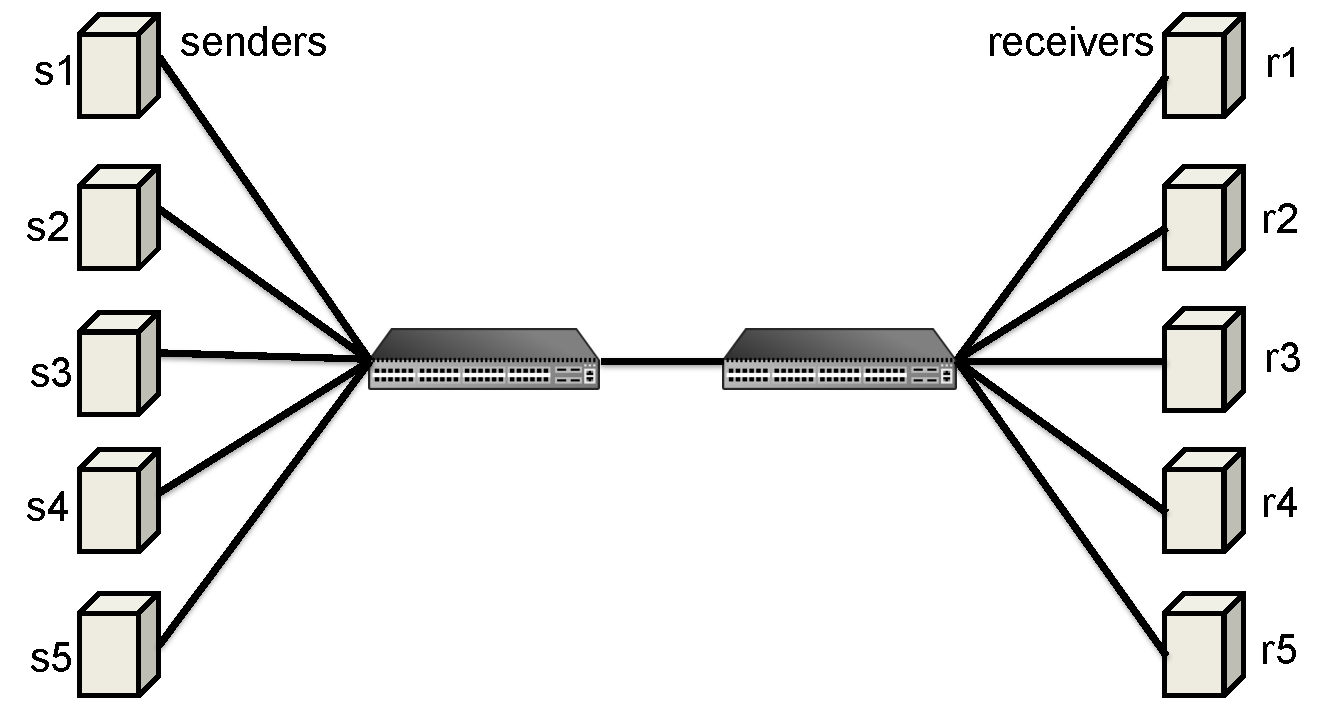
\includegraphics[width=0.7\textwidth]{figures/dumbbell_topology.pdf}
                \caption{Dumbbell topology.}
                \label{dumbbell_topology}
        \end{subfigure}
        \begin{subfigure}[b]{0.5\textwidth}
                \centering
                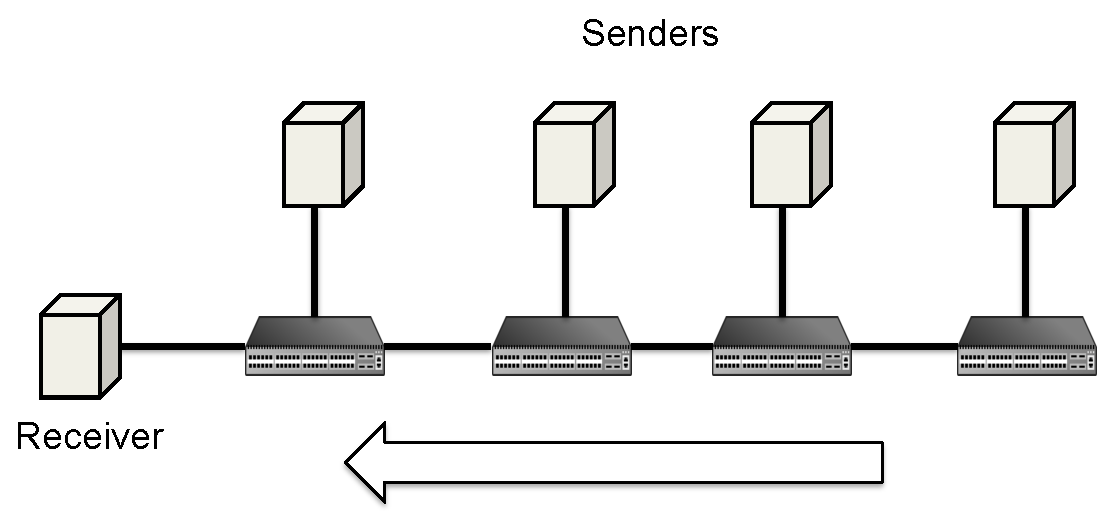
\includegraphics[width=0.7\textwidth]{figures/parkinglot_topology.pdf}
                \caption{Multi-hop, multi-bottleneck (parking lot) topology.}
                \label{parkinglot_topology}
        \end{subfigure}
	\caption{Experiment topologies in microbenchmarks (\cref{micro}).}
	\label{microbenchmarks_topology}
\end{figure}	

%%%coexistence %%%
\begin{figure}[th]
        \centering
        \begin{subfigure}[b]{0.225\textwidth}
                \centering
                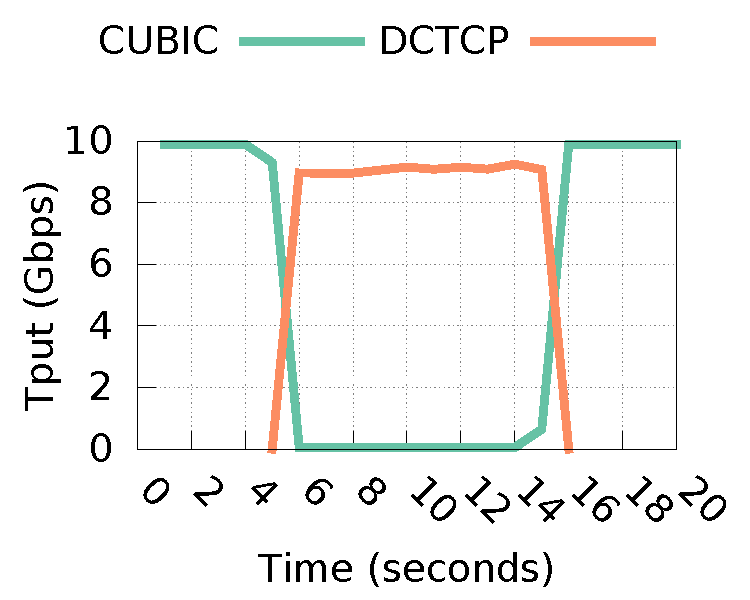
\includegraphics[width=\textwidth]{figures/micro2flows/coexitence/cubic_dctcp_coexistence_official.pdf}
                \caption{Default}
                \label{coexistence_tput_ovs}
        \end{subfigure}
        \begin{subfigure}[b]{0.225\textwidth}
                \centering
                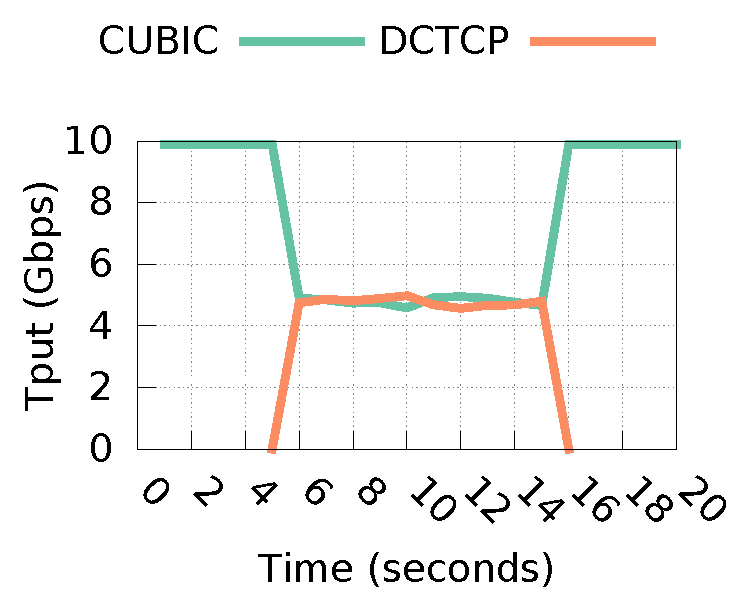
\includegraphics[width=\textwidth]{figures/micro2flows/coexitence/cubic_dctcp_coexistence_acdctcp.pdf}
                \caption{\acdc{}}
                \label{coexistence_tput_ovsdctcp}
        \end{subfigure}
        \caption{(a) CUBIC gets little throughput when competing with DCTCP.
		 (b) With \acdc{}, CUBIC and DCTCP flows get fair share.}
        \label{coexistence_tput}
\end{figure}


\begin{figure}[th]
        \centering
  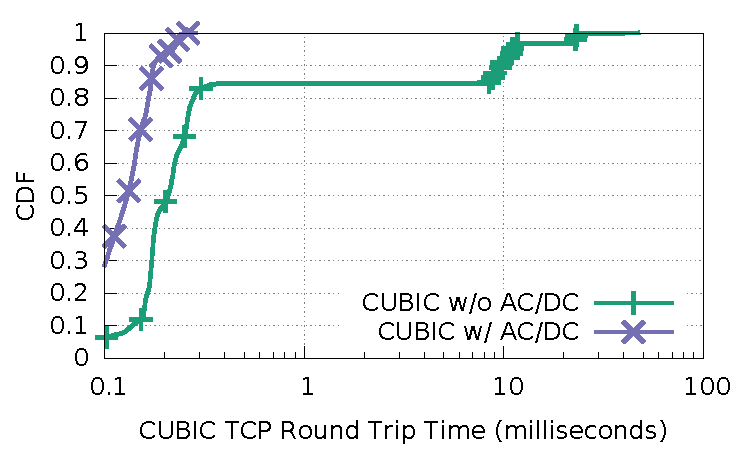
\includegraphics[width=0.45\textwidth]{figures/micro2flows/coexitence/sockperf_and_droprate/coexistence_sockperf.pdf}
        \caption{
		CUBIC traffic experiences very high TCP RTT when competing with DCTCP (packet drop rate is 0.18\%). 
		LiquidSwitch fixes this problem (packet drop rate is 0\%).
		}
        \label{coexistence_sockperf_droprate}
\end{figure}

%%%%%%%%%%%%%%% text for coexistence %%%%%%%%%%
%%%%%%%%%start text in microbenchmark section
We first evaluate \acdc{}'s performance using a set of microbenchmarks.
The microbenchmarks are conducted on topologies shown in Figure~\ref{microbenchmarks_topology}.

\tightparagraph{ECT and non-ECT coexistence}
\cite{judd2015nsdi,wu2012tuning} observed that ECT and non-ECT do not coexist well---switches
drop non-ECT packets when the queue length is (even slightly) larger than the predefined
marking threshold.
We conduct an experiment to validate this and demonstrate how \acdc{} supports ECT and non-ECT coexistence.
Two competing flows (one pair uses CUBIC, the other uses DCTCP) traverse the same bottleneck link in Figure~\ref{dumbbell_topology}.
Figure~\ref{coexistence_tput_ovs} shows that CUBIC's throughput is very poor when it is
mixed with DCTCP traffic using Default scheme. With \acdc{}, CUBIC and DCTCP flows get fair share (Figure~\ref{coexistence_tput_ovsdctcp}).
Figure~\ref{coexistence_sockperf_droprate} shows that CUBIC's TCP RTT is extremely high
because switches drops non-ECT packets (drop rate is 0.18\%) even with there is light congestion 
and CUBIC may need to transmit the dropped
packets for multiple times.
On the other hand, \acdc{} encodes every non-ECT packet into ECT packet and
undo the ECT marking properly when it arrives at the receiver host, so the switches do not discriminate
CUBIC packets. Furthermore, \acdc{} enforces DCTCP-like congestion control in the virtualization layer
by modifying RWND field in the TCP header, so all the TCP variants react to the extent of network
congestion such that the queue occupancy in the switch is small (drop rate is 0\%).
Another method to handle the ECT and non-ECT coexistence issue is to
put ECT and non-ECT flows into different queues and apply different AQM schemes~\cite{judd2015nsdi}.
However, two limitations restrict the applicability of such an approach.
First, in multi-tenant datacenters, it is not always easy (if not impossible) to
know which congestion control algorithm the tenant stack is using.
Second, non-ECT traffic still suffer from huge queueing latency.
In summary, \acdc{} enforces a unified low latency congestion control algorithm for all TCP variants.
It gives low latency and throughput fairness properties to all kinds of TCP traffic.
\emph{\acdc{} makes low latency possible in production data center networks where
incremental deployment is the norm and transport diversity must be supported}.


%%compare with CUBIC defalt and DCTCP test %%%
%% two flow case
\iffalse
\begin{figure}[!htb]
        \centering
  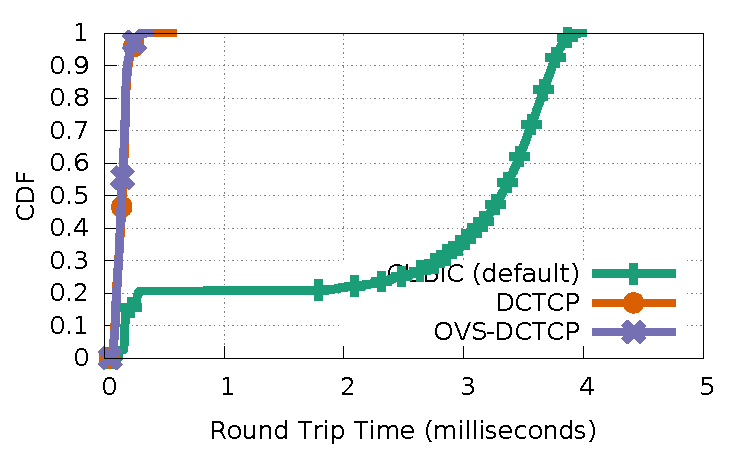
\includegraphics[width=0.45\textwidth]{figures/micro2flows/cubic_ours_dctcp_sockperf.pdf}
        \caption{Compare OVS-DCTCP with CUBIC default and DCTCP. Two flows.
		CUBIC default's throughput is 4.9Gbps. DCTCP 4.9Gbps, OVS-DCTCP 4.8Gbps.}
        \label{compare_cubic_dctcp_twoflows}
\end{figure}
\fi

%%how close our RWND is to DCTCP's CWND
\begin{figure}[!htb]
        \centering
        \begin{subfigure}[b]{0.225\textwidth}
                \centering
                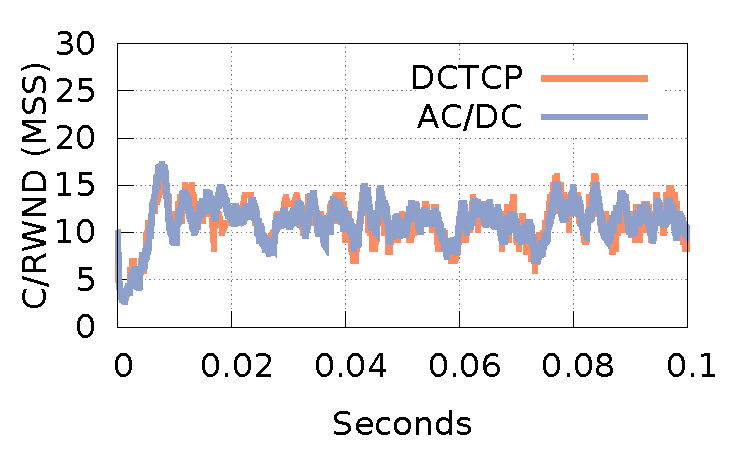
\includegraphics[width=\textwidth]{figures/cwnd_rwnd/newpara_refine/mtu1500_5flows_1/measure_cwnd_rwnd_gap_15k_5flows_0sec_100msec.pdf}
                \caption{MTU1500: first 100 msec starting from second 0.}
                \label{cwnd_rwnd_1500_0sec}
        \end{subfigure}
        \begin{subfigure}[b]{0.225\textwidth}
                \centering
                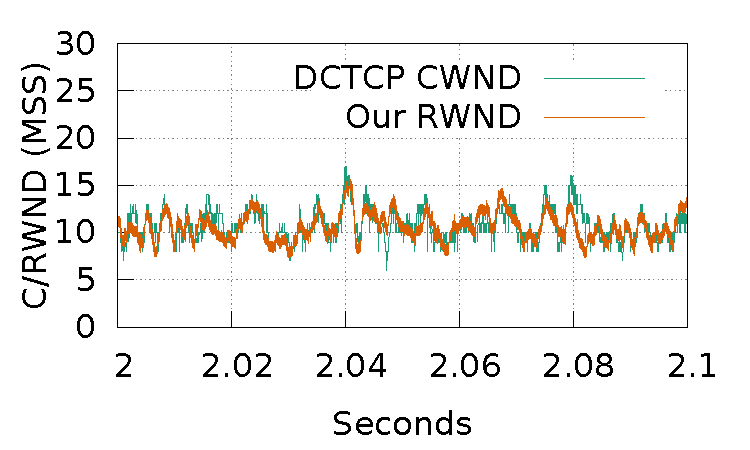
\includegraphics[width=\textwidth]{figures/cwnd_rwnd/newpara_refine/mtu1500_5flows_1/measure_cwnd_rwnd_gap_15k_5flows_2sec_100msec.pdf}
                \caption{MTU1500: first 100 msec starting from second 2.}
                \label{cwnd_rwnd_1500_2sec}
        \end{subfigure}

	\begin{subfigure}[b]{0.225\textwidth}
                \centering
                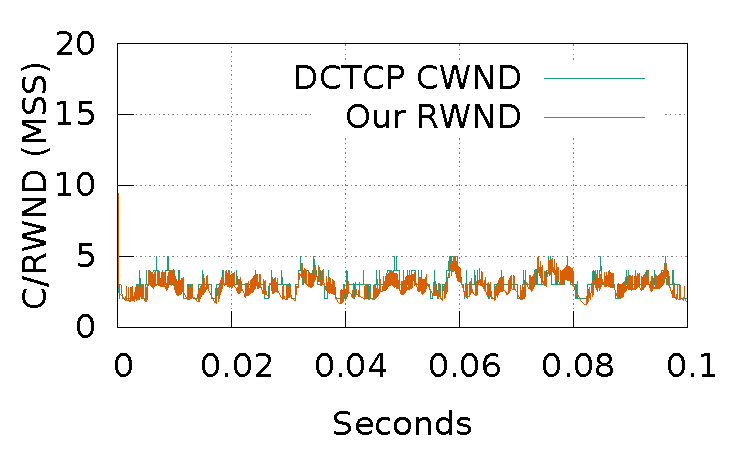
\includegraphics[width=\textwidth]{figures/cwnd_rwnd/newpara_refine/mtu9000_5flows_1/measure_cwnd_rwnd_gap_9k_5flows_0sec_100msec.pdf}
                \caption{MTU9000: first 100 msec starting from second 0.}
                \label{cwnd_rwnd_9000_0sec}
        \end{subfigure}
        \begin{subfigure}[b]{0.225\textwidth}
                \centering
                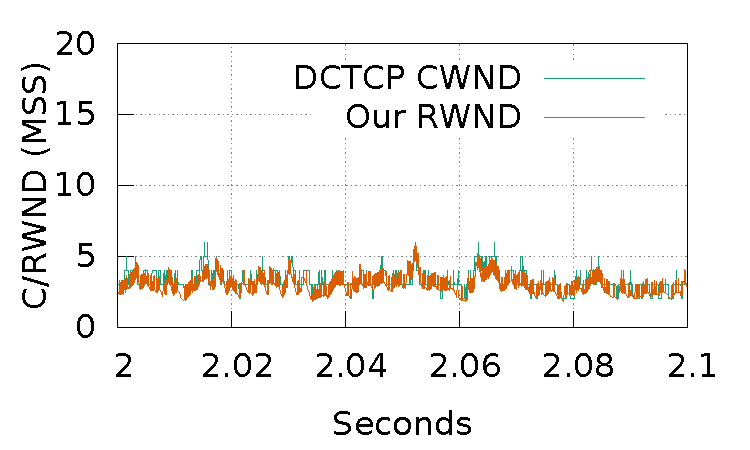
\includegraphics[width=\textwidth]{figures/cwnd_rwnd/newpara_refine/mtu9000_5flows_1/measure_cwnd_rwnd_gap_9k_5flows_2sec_100msec.pdf}
                \caption{MTU9000: first 100 msec starting from second 2.}
                \label{cwnd_rwnd_9000_2sec}
        \end{subfigure}
        \caption{Ours RWND closely tracks the CWND offered by DCTCP. We run DCTCP and output our running RWND value
		without enforcing it in TCP ACKs. Dumbbell topology. Microview. CWND trace captured by ``tcpprobe'' and
		RWND logged by OVS's datapath kernel module. Then we align the two kinds of traces by timestamp and sequence numbers.}
        \label{compare_cwnd_rwnd}
\end{figure}


%%who limits TCP throughput, CWND or RWND? CUBIC
\begin{figure}[!htb]
        \centering
        \begin{subfigure}[b]{0.225\textwidth}
                \centering
                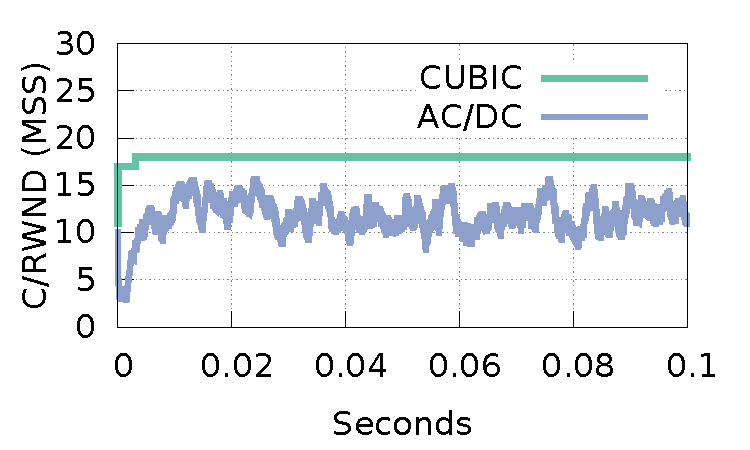
\includegraphics[width=\textwidth]{figures/cwnd_rwnd2/mtu1500_cubic/cubic_measure_cwnd_rwnd_gap_15k_5flows_0sec_100msec.pdf}
                \caption{MTU1500: first 100 msec starting from second 0.}
                \label{who_limits_cwnd_rwnd_1500_0sec}
        \end{subfigure}
        \begin{subfigure}[b]{0.225\textwidth}
                \centering
                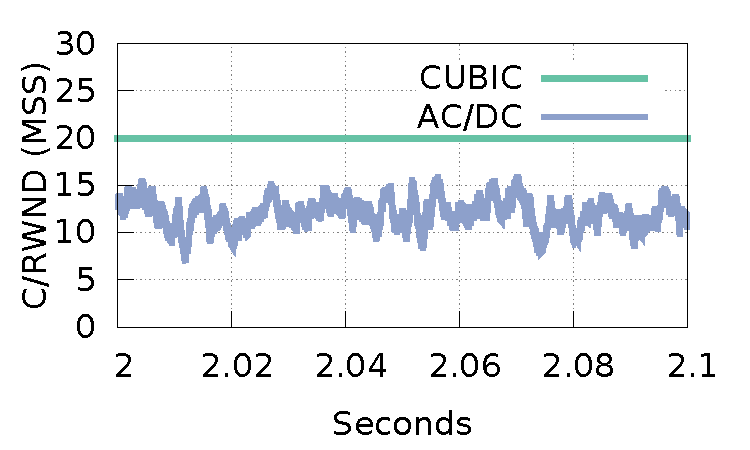
\includegraphics[width=\textwidth]{figures/cwnd_rwnd2/mtu1500_cubic/cubic_measure_cwnd_rwnd_gap_15k_5flows_2sec_100msec.pdf}
                \caption{MTU1500: first 100 msec starting from second 2.}
                \label{who_limits_cwnd_rwnd_1500_2sec}
        \end{subfigure}

        \begin{subfigure}[b]{0.225\textwidth}
                \centering
                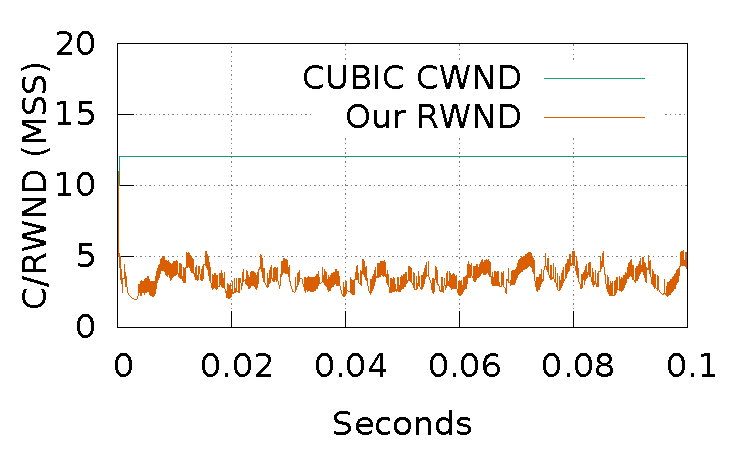
\includegraphics[width=\textwidth]{figures/cwnd_rwnd2/mtu9000_cubic/cubic_measure_cwnd_rwnd_gap_9k_5flows_0sec_100msec.pdf}
                \caption{MTU9000: first 100 msec starting from second 0.}
                \label{who_limits_cwnd_rwnd_9000_0sec}
        \end{subfigure}
        \begin{subfigure}[b]{0.225\textwidth}
                \centering
                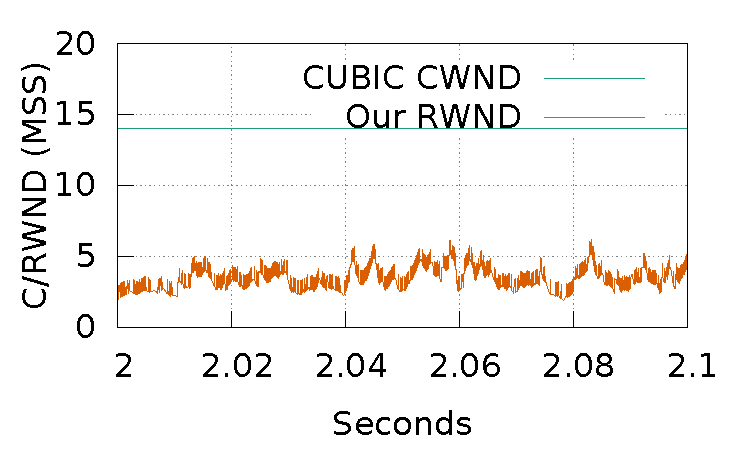
\includegraphics[width=\textwidth]{figures/cwnd_rwnd2/mtu9000_cubic/cubic_measure_cwnd_rwnd_gap_9k_5flows_2sec_100msec.pdf}
                \caption{MTU9000: first 100 msec starting from second 2.}
                \label{who_limits_cwnd_rwnd_9000_2sec}
        \end{subfigure}
        \caption{Who limits TCP throughput? CWND or RWND? We run CUBIC on top and output our running RWND value
                while enforcing it in TCP ACKs. Dumbbell topology. Microview. CWND trace captured by ``tcpprobe'' and
                RWND logged by OVS's datapath kernel module. Then we align the two kinds of traces by timestamp and sequence numbers.}
        \label{who_limits_compare_cwnd_rwnd}
\end{figure}


%%how close our RWND is to DCTCP's CWND
\begin{figure}[!htb]
        \centering
        \begin{subfigure}[b]{0.225\textwidth}
                \centering
                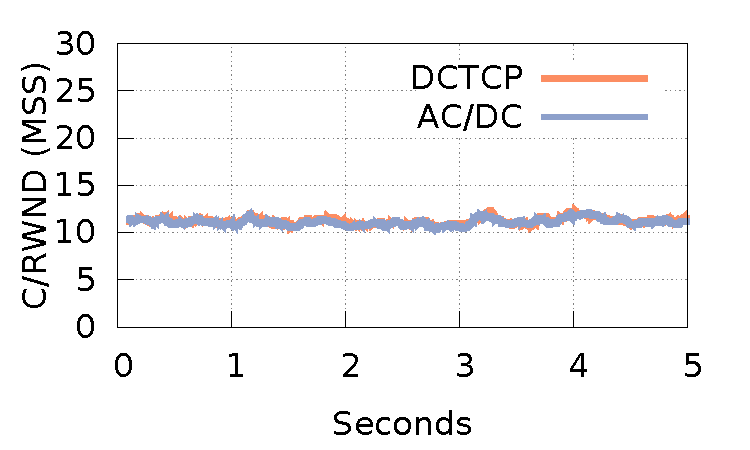
\includegraphics[width=\textwidth]{figures/cwnd_rwnd/moving-ave/measure_cwnd_rwnd_gap_15k_5flows_ave100.pdf}
                \caption{MTU1500: Moving average over 100 ms window.}
                \label{cwnd_rwnd_1500_0sec}
        \end{subfigure}
        \begin{subfigure}[b]{0.225\textwidth}
                \centering
                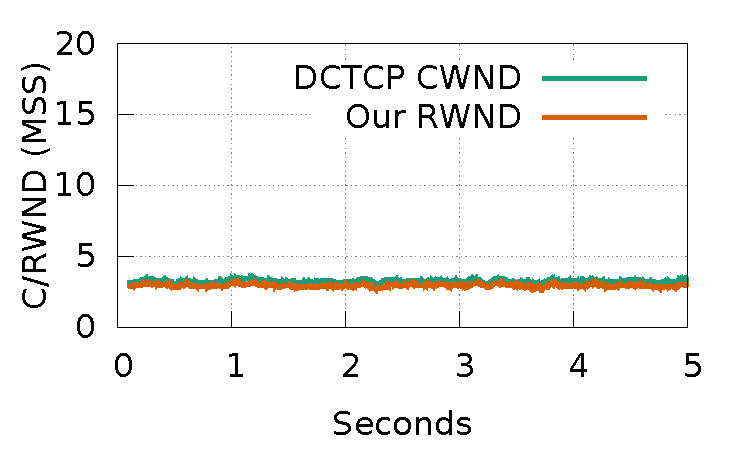
\includegraphics[width=\textwidth]{figures/cwnd_rwnd/moving-ave/measure_cwnd_rwnd_gap_9k_5flows_ave100.pdf}
                \caption{MTU9000: Moving average over 100 ms window.}
                \label{cwnd_rwnd_1500_2sec}
        \end{subfigure}

        \caption{Ours RWND closely tracks the CWND offered by DCTCP. We run DCTCP and output our running RWND value
                without enforcing it in TCP ACKs. Dumbbell topology. CWND trace captured by ``tcpprobe'' and
                RWND logged by OVS's datapath kernel module. Then we align the two kinds of traces by timestamp and sequence numbers.
		Moving average over 100 ms windows presented.}
        \label{compare_cwnd_rwnd_ave}
\end{figure}


%%% other TCP variants %%%
\begin{table*}[!htb]
\begin{center}
\begin{tabular}{ |c|c|c|c|c|c| }
 \hline
 CC variants & 50$^{th}$ percentile TCP RTT ($\mu$s) & 99.9$^{th}$ percentile TCP RTT ($\mu$s) & Throughput (Gbps) \\
 \hline
 CUBIC*  & 3283 & 3714 & 1.89 \\
 DCTCP*  & 136  & 342  & 1.88 \\
 \hline
 \hline
 %%INIT 5, STEP 0.75
 %CUBIC & 142 & 362 & 1.86 \\
 %New Reno  & 136 & 348 & 1.87 \\
 %DCTCP (clear ECE) & 139 & 337 & 1.86 \\
 %DCTCP (keep ECE) &  141 & 367 &  1.85\\
 %CUBIC+ECN (clear ECE) & 138 & 372 & 1.86\\
 %CUBIC+ECN (keep ECE) &  112 & 338 & 1.70  \\

 %% INIT 10, STEP 1.0
 CUBIC & 139 & 359 & 1.87 \\
 New Reno  & 145 & 346 & 1.87 \\
 DCTCP (clear ECE) & 137 & 343 & 1.87 \\
 DCTCP (keep ECE) &  144 & 360 &  1.86 \\
 CUBIC+ECN (clear ECE) & 135 & 343 & 1.87\\
 CUBIC+ECN (keep ECE) &  121 & 316 & 1.50 \\
 \hline
\end{tabular}
\caption{OVS-DCTCP works with various kinds of congestion control variants.
        CUBIC*: TCP CUBIC + official OVS, switch ECN/WRED marking off.
        DCTCP*: DCTCP + official OVS, switch ECN/WRED marking on. MTU = 1500B}
\label{other_cc_variants_1500}
\end{center}
\end{table*}


\begin{table*}[!htb]
\begin{center}
\begin{tabular}{ |c|c|c|c|c|c| }
 \hline
 CC variants & 50$^{th}$ percentile TCP RTT ($\mu$s) & 99.9$^{th}$ percentile TCP RTT ($\mu$s) & Throughput (Gbps) \\
 \hline
 %CUBIC & 148 & 299 & 4.8  \\
 %New Reno   & 142 & 336 & 4.8 \\
 %DCTCP (clear ECE) & 142 & 318 & 4.8 \\
 %DCTCP (keep ECE) & 144 & 403  & 4.7 \\
 %CUBIC+ECN (clear ECE) & 151 & 301 & 4.8\\
 %CUBIC+ECN (keep ECE) &  119 & 307 & 4.0  \\
 CUBIC*  & 3408 & 3976 & 1.98 \\
 DCTCP*  & 158  & 362  & 1.97 \\ 
 \hline
 \hline 
 CUBIC & 154 & 343 & 1.94  \\
 New Reno   & 156 & 324 & 1.94 \\
 DCTCP (clear ECE) & 155 & 355 & 1.94 \\
 DCTCP (keep ECE) & 155 & 368  & 1.93 \\
 CUBIC+ECN (clear ECE) & 158 & 359 & 1.94\\
 CUBIC+ECN (keep ECE) &  153 & 309 & 1.92  \\
 \hline

\end{tabular}
\caption{OVS-DCTCP works with various kinds of congestion control variants.
        CUBIC*: TCP CUBIC + official OVS, switch ECN/WRED marking off.
        DCTCP*: DCTCP + official OVS, switch ECN/WRED marking on. MTU = 9000B} 
\label{other_cc_variants}
\end{center}
\end{table*}


%%%convergence %%%
\begin{figure}[!htb]
        \centering
  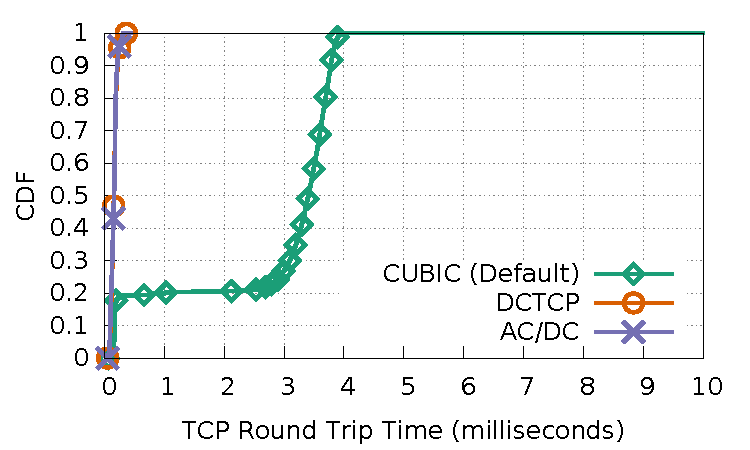
\includegraphics[width=0.45\textwidth]{figures/convergence/flowcontrolOFF_sockperf/convergence_test_sockperf.pdf}
        \caption{Compare OVS-DCTCP with CUBIC default and DCTCP. TCP RTT (sockperf). RTO\_{min} is 10 ms in all of our experiments. Dumbbell topology.}
        \label{sockperf_convergence}
\end{figure}


\begin{figure*}[t]
        \centering
        \begin{subfigure}[b]{0.33\textwidth}
                \centering
		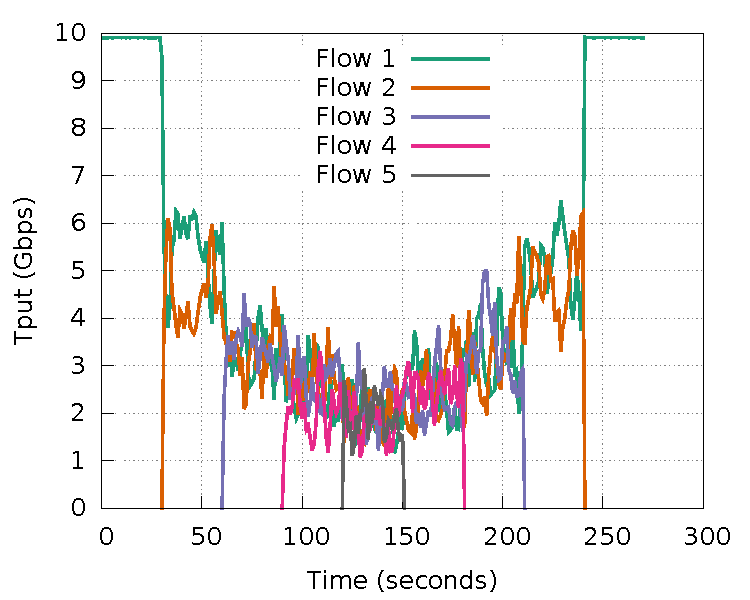
\includegraphics[width=\textwidth]{figures/convergence/flowcontrolOFF/tcp_flowcontrolOFF_convergence.pdf}
		\caption{TCP CUBIC convergence test.}
        	\label{cubic_convergence}	
	\end{subfigure}
	\begin{subfigure}[b]{0.33\textwidth}
                \centering
		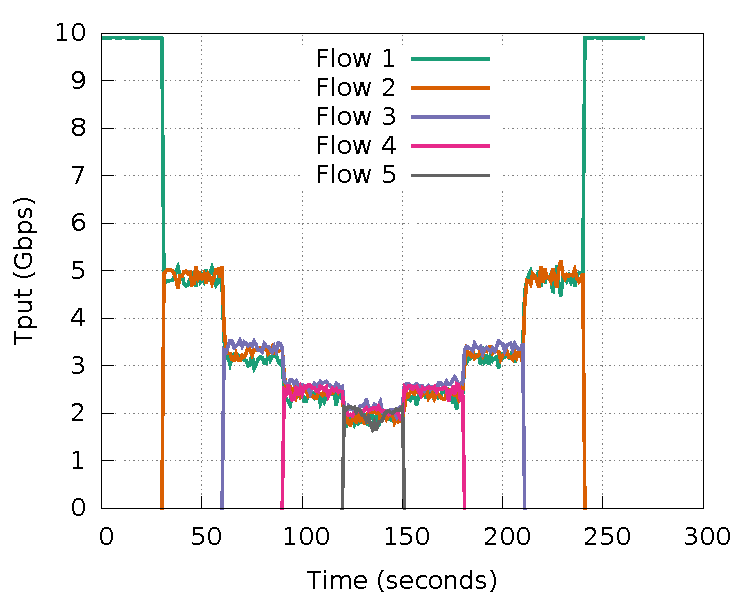
\includegraphics[width=\textwidth]{figures/convergence/flowcontrolOFF/dctcp_flowcontrolOFF_convergence.pdf}
		\caption{DCTCP convergence test.}
        	\label{dctcp_convergence}
	\end{subfigure}
	\begin{subfigure}[b]{0.33\textwidth}
                \centering
		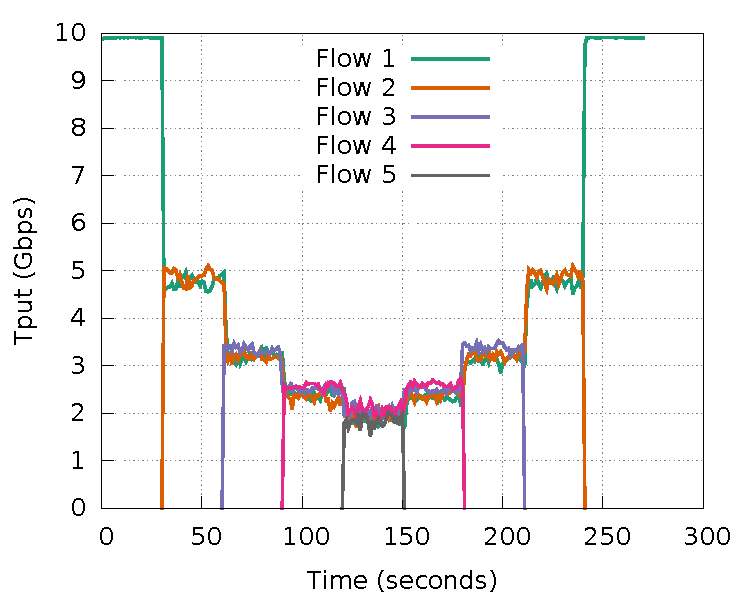
\includegraphics[width=\textwidth]{figures/convergence/flowcontrolOFF/ovsdctcp_flowcontrolOFF_convergence.pdf}
		\caption{OVS-DCTCP convergence test.}
        	\label{ovsdctcp_convergence}
	\end{subfigure}
	\caption{Convergence tests. TCP CUBIC's drop rate is 0.17\% while DCTCP and OVS-DCTCP is 0\%.
		A note on CUBIC: as explained by~\cite{judd2015nsdi}, its stability, convergence and fairness issue
		is caused by receive buffer auto-tuning of the OS and it can be fixed by manually 
		setting the TCP socket buffer size. We confirmed this finding on our testbed. 
		We share the same view that ``achieving proper receive buffer sizing, however, 
		is much more difficult under TCP due to the massive dynamic range of latencies''---another 
		motivation for unified low latency transport enforcement for all TCP variants.
		}
	\label{convergence_test}
\end{figure*}

\begin{figure*}[!htb]
        \centering
        \begin{subfigure}[b]{0.24\textwidth}
                \centering
                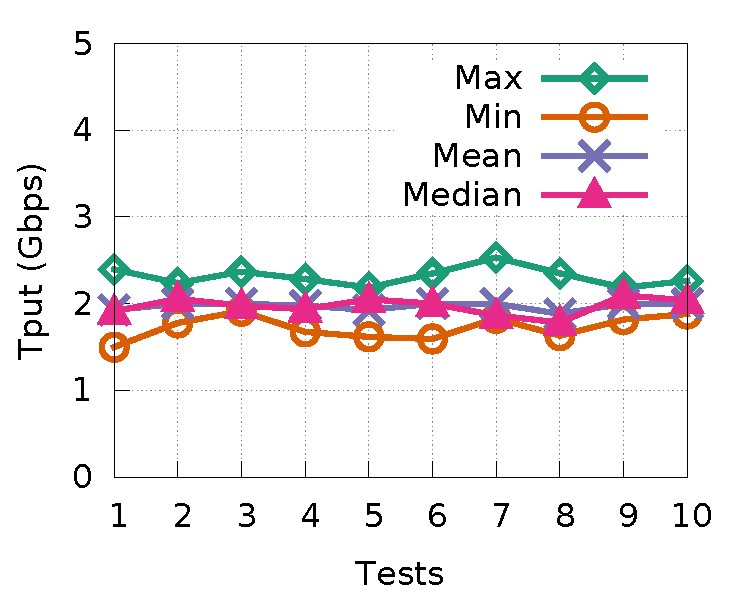
\includegraphics[width=\textwidth]{figures/tput_fairness/default_all_cubic_tput.pdf}
                \caption{All CUBIC.}
                \label{fairness_all_cubic}
        \end{subfigure}
        \begin{subfigure}[b]{0.24\textwidth}
                \centering
                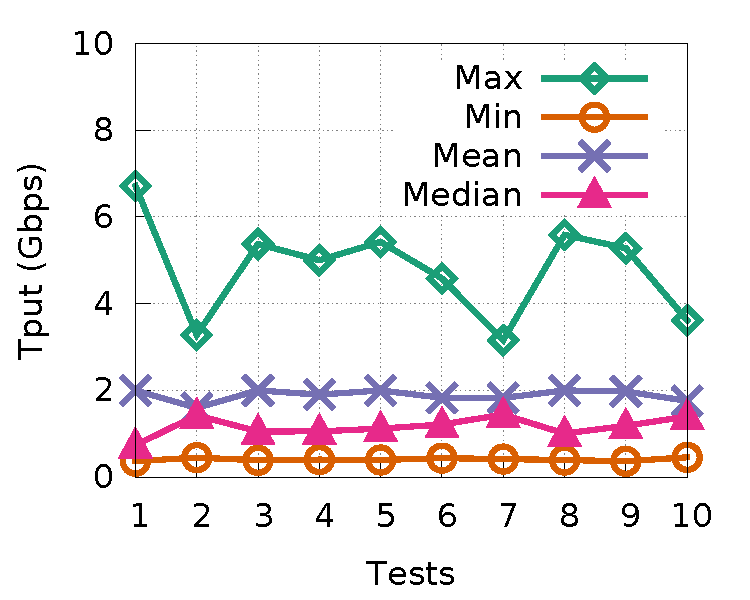
\includegraphics[width=\textwidth]{figures/tput_fairness/default_5CC_tput.pdf}
                \caption{5 different CCs.}
                \label{fairness_5CC}
        \end{subfigure}
        \begin{subfigure}[b]{0.24\textwidth}
                \centering
                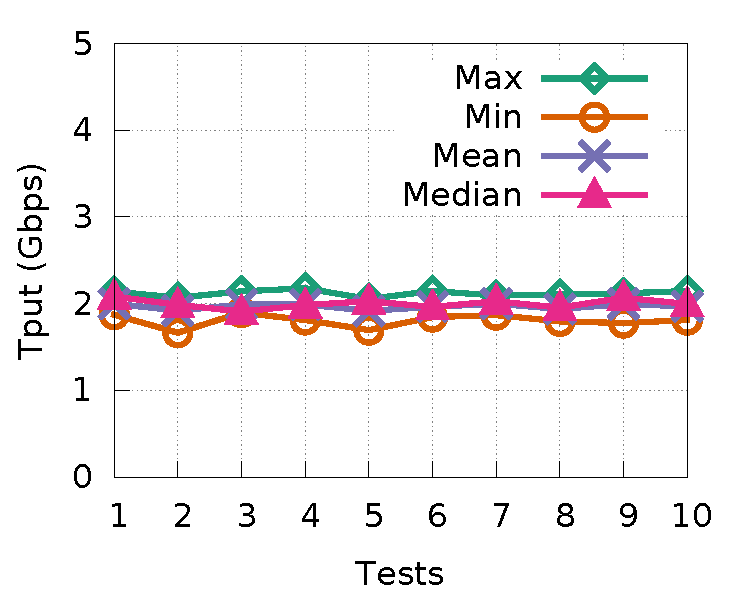
\includegraphics[width=\textwidth]{figures/tput_fairness/liquid_5CC_tput.pdf}
                \caption{5 different CCs with our logic.}
                \label{fairness_5CC_with_ours}
        \end{subfigure}
        \begin{subfigure}[b]{0.24\textwidth}
                \centering
                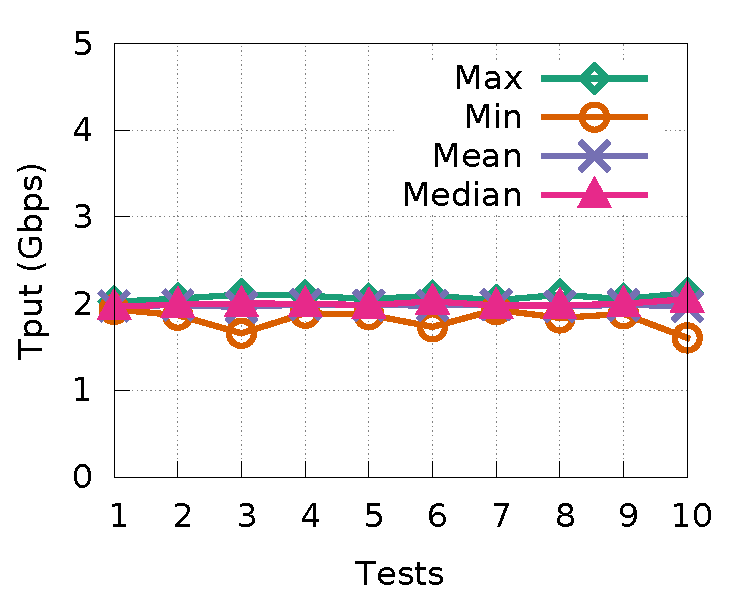
\includegraphics[width=\textwidth]{figures/tput_fairness/ecn_all_dctcp_tput.pdf}
                \caption{All DCTCP.}
                \label{fairness_5CC_with_ours}
        \end{subfigure}
	\caption{Our logic can help improve TCP variants' throughput fairness. 
		receive buffer auto-tuning on.	
		5 different CCs are: TCP CUBIC~\cite{ha2008cubic}, TCP Illinois~\cite{liu2008tcp}, 
		TCP HighSpeed~\cite{RFC3649}, 
		TCP New Reno~\cite{RFC3782} and TCP Vegas~\cite{Brakmo1994}.	     
		50th and 99.9$^{th}$ percentile TCP RTTs for all CUBIC, 5 different CCs, 5 different CCs with
		our logic and all DCTCP are: 3.5 msec, 3.9msec; 3.4 msec, 4.0 msec; 146 $\mu$s, 306 $\mu$s;
		147 $\mu$s, 317 $\mu$s. Both ours and DCTCP offer a Jain's fairness index greater than 0.99. }
 	\label{tput_fairness_coexistence}
\end{figure*}	

\begin{figure}[!htb]
        \centering
  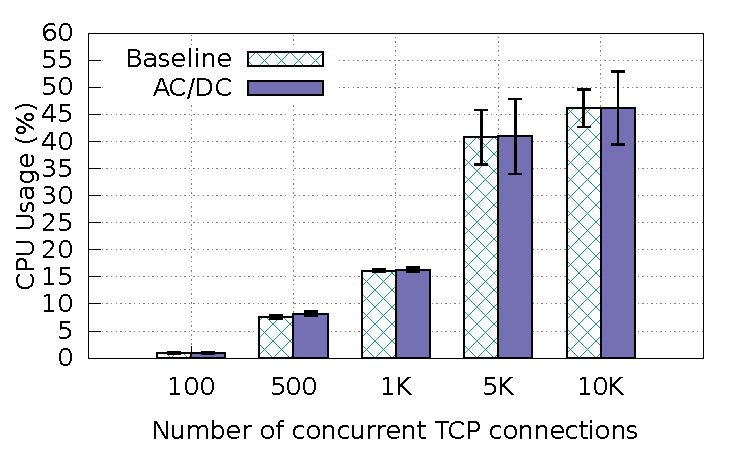
\includegraphics[width=0.45\textwidth]{figures/overhead/sender_15k_compare_cpu_witherrbar.pdf}
        \caption{CPU overhead: sender side (1.5K MTU). The 10G NIC is saturated when there are more than 1K TCP connections.
		CPU usage refers to the CPU usage of the whole server (12 Intel(R) Xeon(R) CPU E5649@2.53GHz processors), 
		measured by ``sar (sysstat)''.}
        \label{cpu_overhead_sender_15k}
\end{figure}

\begin{figure}[!htb]
        \centering
  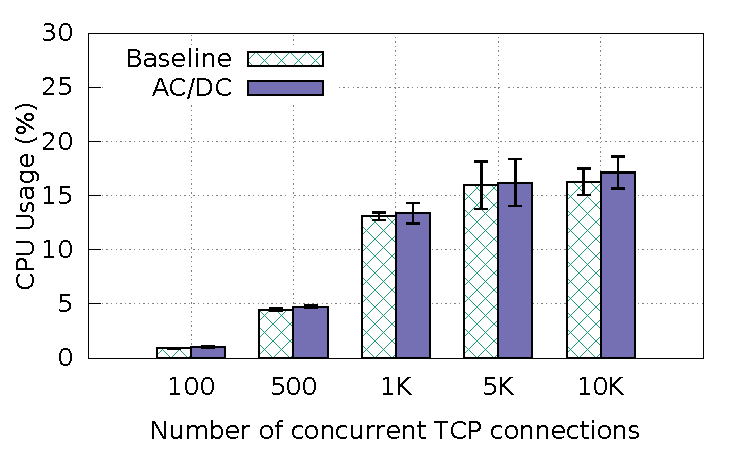
\includegraphics[width=0.45\textwidth]{figures/overhead/receiver_15k_compare_cpu_witherrbar.pdf}
        \caption{CPU overhead: receiver side (1.5K MTU). The 10G NIC is saturated when there are more than 1K TCP connections.
		CPU usage refers to the CPU usage of the whole server (12 Intel(R) Xeon(R) CPU E5649@2.53GHz processors) 
		measured by ``sar (sysstat)''.}
        \label{cpu_overhead_receiver_15k}
\end{figure}

\begin{figure}[!htb]
        \centering
  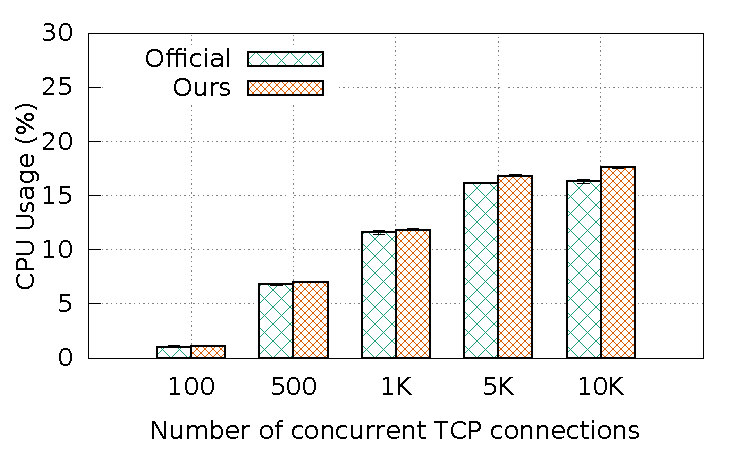
\includegraphics[width=0.45\textwidth]{figures/overhead/sender_9k_compare_cpu_witherrbar.pdf}
        \caption{CPU overhead: sender side (9K MTU). The 10G NIC is saturated when there are more than 1K TCP connections.
		CPU usage refers to the CPU usage of the whole server (12 Intel(R) Xeon(R) CPU E5649@2.53GHz processors)
                measured by ``sar (sysstat)''.}
        \label{cpu_overhead_sender_9k}
\end{figure}

\begin{figure}[!htb]
        \centering
  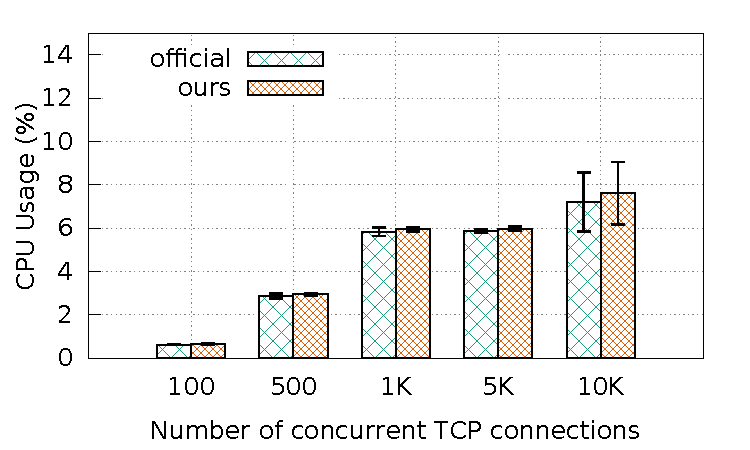
\includegraphics[width=0.45\textwidth]{figures/overhead/receiver_9k_compare_cpu_witherrbar.pdf}
        \caption{CPU overhead: receiver side (9K MTU). The 10G NIC is saturated when there are more than 1K TCP connections.
		CPU usage refers to the CPU usage of the whole server (12 Intel(R) Xeon(R) CPU E5649@2.53GHz processors)
                measured by ``sar (sysstat)''}
        \label{cpu_overhead_receiver_9k}
\end{figure}

%%%%%%%%%start text in microbenchmark section

\tightparagraph{Compare with TCP (default) and DCTCP}
\acdc{} achieves similar throughput with TCP CUBIC and DCTCP. When 5 flows compete
for a 10Gbps bottleneck, each flow get around 1.94Gbps with \acdc{} while TCP CUBIC
and DCTCP achieve 1.98Gbps and 1.97Gbps, respectively. \acdc{} achieves comparable TCP RTT compared
with DCTCP and significantly outperforms TCP CUBIC (Figure~\ref{sockperf_convergence}).

How close we are from DCTCP? Figure~\ref{compare_cwnd_rwnd}.

\tightparagraph{Support various kinds of congestion control (CC) variants}
Table~\ref{other_cc_variants} show that \acdc{} can work with various kinds of congestion control variants that
are defined by tenants.
It can also help over-conservative congestion control schemes
(\eg{}, CUBIC with ECN support) get better throughput via cleaning ECE bit in TCP ACKs while
still keeping latency low.

\tightparagraph{Convergence and fairness}
Figure~\ref{convergence_test} shows that \acdc{} can converge quickly. Both \acdc{} and DCTCP
have a Jain's fairness index greater than 0.99.
%Figure~\ref{sockperf_convergence} shows that \acdc{}
%has very good TCP RTT performance.


\tightparagraph{Different MTU sizes}
We set MTU size to 1500 bytes and run the tests on the dumbbell topology (Figure~\ref{dumbbell_topology})
with 5 flows competing for
a 10G bottleneck link. \acdc{} gets 1.87Gbps average flow throughput. DCTCP gets 1.88Gbps average flow throughput. 
Both have a Jain's fairness index greater than 0.99. TCP CUBIC gets 1.89 average flow throughput and a fairness index of 0.85.
The 50$^{th}$ and 99.9$^{th}$ percentile TCP RTT for \acdc{} (DCTCP, CUBIC) are 139$\mu$s (136$\mu$s, 3.2ms) and
359$\mu$s (342$\mu$s, 3.7ms), respectively.

\tightparagraph{Multi-hop, multi-bottleneck topology}
We test \acdc{}'s performance on a parking lot topology as shown in
Figure~\ref{parkinglot_topology}.
We start background elephant flows from
four senders to one receiver. The elephant flows traverse different number of
bottleneck links. We measure each flow's throughput and TCP RTT.
Our results show that for both DCTCP and \acdc{}, each flow can get around 2.45Gbps
throughput, with a Jain's fairness index greater than 0.99.
CUBIC's average throughput is 2.48Gbps, and its fairness index is 0.94.
The 50$^{th}$ and 99.9$^{th}$ percentile TCP RTT for
\acdc{} (DCTCP, default CUBIC) are 124$\mu$s (136$\mu$s, 3.3msec) and
279$\mu$s (301$\mu$s, 3.9msec), respectively.

TCP-Bolt~\cite{stephens2014practical} and DCQCN~\cite{zhu2015congestion} found
that Data Center Bridging (DCB) can have throughput unfairness and 
increased queueing (bufferbloat) issues and such issues can be solved by utilizing
ECN (like DCTCP). We anticipate our scheme can also work in DCB.

\tightparagraph{Little CPU and memory overhead}
In our implementation, first we leverage the Read-Copy-Update (RCU)~\cite{guniguntala2008read} enabled hash tables
to keep per-flow states (such as ``snd\_una'' and ``snd\_nxt''). RCU technique is also employed by
Open vSwitch's kernel datapath and it helps improve processing speed for ``read-heavy''
workloads (\eg{}, interesting new flows is less frequent than looking-up existing flows) on
shared-memory multiprocessor systems.
Second, \acdc{} processes on ``segment'' level instead of ``packet'' level due to
NIC offloading features (TSO at the sender side and GRO/LRO at the receiver side).
Third, we also leverage the NIC checksumming offloading feature such that
we do not need to compute checksums after we change TCP/IP header fields.
Our microbenchmarks show that \acdc{} incurs very little additional CPU overhead (less than 2\%) to
support 10Gbps line-rate, even it is fully implemented in software.
We are currently implementing \acdc{} on Cavium's programmable NICs~\cite{cavium-nic},
where we can entirely offload the computational overhead to hardware. Therefore, we believe
\acdc{} can support even higher line rates (\eg{}, 40Gbps).
In our implementation, each TCP connection takes 320 bytes in the hash tables,
so it takes around 3.2MB even there are 10K connections.

Figure~\ref{cpu_overhead_sender_15k} and Figure~\ref{cpu_overhead_receiver_15k}.
Figure~\ref{cpu_overhead_sender_9k} and Figure~\ref{cpu_overhead_receiver_9k}.
